\chapter{Experiment}%
\label{cha:experiment}

Now, when important theoretical concerns are discussed we will move to experiment with NNs on EEG brain data. This chapter will describe used dataset and methods with NN models during experiment. Achieved results are presented as last part and later discussed.

This experiment was based on paper \cite{varekap300}. The aim was to classify retrieved brainwave data to classes of target and non-target numbers (meaning explained in Section~\ref{sec:dataset}) with supervised learning of NNs. (Section~\ref{sec:supervised_ann}, Section~\ref{sec:supervised_snn}) In the original paper, author was able to achieve accuracy of 62-64\% when classifying single-trial components (one 1200 ms long stimuli sample), but when averaging of the components was applied, the accuracy increased to 76-79\%. The author main used NN model was 2D Convolutional ANN.

Classification with both ANNs and SNNs, together with both single-trial data and data averaging, was the goal during this experiment

%
% DATASET
%

\section{Dataset}%
\label{sec:dataset}

Dataset consists of P300 brainwaves retrieved from 250 school-age children (138 males and 112 females). Authors of the dataset visited elementary and secondary schools and let children participate in an experiment. The children were asked to choose a number in a range of 1 to 9 during the experiment. The chosen number is referred to as the \textit{target} number and other numbers are referred to as the \textit{non-target} numbers. After a participant's choice, they were show a random number for one second long interval and had to focus, when their number appeared. Their brain waves were recorded from three channels (Fz, Cz, Pz) in total, 200 ms before start of the stimuli and 1000 ms during it. The result is 1200 ms long sample in three vectors for one stimulation. Total amount of samples is 11~532. Participants were stimulated with multiple numbers within a few minutes.

How dataset was processed during the experiment is described in a following section. Dataset is available at \cite{dataset} and thoroughly described in \cite{dataset-article}.

%
% METHODS
%

\section{Methods}%
\label{sec:methods}

For the experiment, Tensorflow (Subsection~\ref{sub:tensorflow}) and NengoDL (Subsection~\ref{ssub:nengodl}) were used, due to their good compatibility. Both libraries were used with their Python API. Models were trained and tested on CPU Intel~i5-8300H. Following part describes used pre-processing, neural models and how training was done.

%
% PREPROCESSING & TRAINING
%

\subsection{Pre-processing and training}%
\label{ssec:preproc_train}

The dataset \cite{dataset} can be loaded as a Python dictionary. It is divided into two parts -- part with target numbers under key \texttt{allTargetData} and part with non-target numbers under key \texttt{allNonTargetData}. The data were filtered to remove damaged samples for example after blinking or distractions from surroundings. A threshold for the filtering was set to $100\ \mu V$ from both sides, so all signals with higher value than $100\ \mu V$ or lower than $-100\ \mu V$ were removed. The~samples were labeled afterwards with hot-encoded vector (1,~0) for targets and vector (0,~1) for non-targets. The~signals from all three channels were joined together into one vector with length 3600 (3~$\times$~1200~recorded milliseconds) creating one long signal. Then the matrices of targets and non-targets were concatenated together with their labels, which created a matrix of size $8036 \times 1 \times 3600$ (number of samples $\times$ channels $\times$ number of features).

Above described is data preparation without averaging. As suggested in original paper \cite{varekap300}, averaging helped to increase accuracy of used Convolutional ANN. The~averaging, which is the aim of this experiment, was approached in two ways here.

\begin{enumerate}
	\item Processing version 1 (PV1) averaged consecutive values in a signal with sliding window of size 3, 6 and 9. The channels for this step had to be preserved (they were joined into the shape described above later). The window was gradually iterating over the values in the signal and was creating new values. Essentially smoothening the signal. Consequence was shortening the signal by the window size minus one. Using values from the beginning of the signal to average them with the values in the end could create unwanted artifacts, that could lower accuracy -- signal would not be continuous. This was done for all three channels and like this new sample for a one person was created.

		When data were in correct form, they were randomly split in ratio 80\% for training data and 20\% for testing data. And during training, the training data were randomly split in ratio 80\% for actual training data and 20\% for validation data.

	\item Processing version 2 (PV2) was averaging whole samples (the reshaped 3600 long vector) among all people randomly. The amount of samples to average here together was 3, 6, 9, 12 and 15. There was a matrix with random values generated for this approach. The height of the matrix was optional and represented amount of new samples in a training dataset part. The width was the averaging amount. In the rows there were indexes of samples from the original dataset to average. Like this it was possible to create entirely new training dataset with optional size. Therefore, training size was set to 10~000 and then to 20~000 samples. The \textit{original dataset} was used as \textit{testing data}. So~the models were trained on artificial generalized data and were tested on untouched data from a real world.
\end{enumerate}

\textit{Cross-validation} was set to 10, meaning there were 10 different model instances of one NN model (all models are described in Subsection~\ref{sub:nn_models}) and the training data were randomly split 10 times for every new model. After training, test data were given to model for prediction and metrics were collected. Final results (Section~\ref{sec:results}) are averages from all cross-validation iterations.

In the beginning of script there is randomness set to zero value, in order to get reproducible results\footnote{Although, network with LSTM layers does not produce same result after rerun. There is an opened issue on GitHub already (June 2021). \url{{https://github.com/tensorflow/tensorflow/issues/18323}}}. All models were trained for 30 \textit{epochs} with \textit{early stopping} set to value of 5. It means that training will stop, if training loss and validation loss function value will not improve for 5 epochs. Train and test \textit{batch size} was set to 32 for PV1 and 50 for PV2. Small change during the second preprocessing was setting the batch size to 100 for model 4 with LMU neurons -- it performed better that way, so final results in Table~\ref{tab:results_samples_10000} and Table~\ref{tab:results_samples_20000} are from training this way. Collected metrics are \textit{accuracy}, \textit{precision}, \textit{recall}, \textit{F1-score} and \textit{confusion matrix}.

%
% NN MODELS
%

\subsection{NN models}%
\label{sub:nn_models}

There were four NN models used in total. Two ANN models and two SNN models. One SNN was converted from ANN model and the other one was created from scratch with novel LMU neurons (Section~\ref{sub:lmu}). ANN models were compiled with \textit{Adam optimizer} and \textit{binary cross-entropy} loss function. Both ANNs used \textit{ReLU} activation function (Subsection~\ref{sub:relu}) in deep layers and \textit{Softmax} function (Subsection~\ref{sub:softmax}) in the output layer.

Difference of the two ANNs is that the first created contained 1D convolutional layer and 1D average pooling layer, while the second one contained two LSTM layers. As mentioned earlier, in the original paper \cite{varekap300} 2D convolutional layers were used, but in this experiment just 1D convolutional layers were used in order to keep one-dimensionality of brain signal and not to convolve different channel signals together. For second ANN were chosen LSTM layers in order to test performance of Recurrent NN as well, because they achieve very good results with processing 1D data. The architecture of the ANNs can be seen in Figure~\ref{fig:arch_anns}. Implementation and detailed parameters of the Convolutional ANN can be seen in Listing~\ref{list:code_ann1} and the LSTM ANN can be seen Listing~\ref{list:code_ann2}. Summary of used models for better orientation can be found in Table~\ref{tab:models}.

\begin{table}[ht!]
	\centering
	\begin{tabular}{c c c c}
		\hline
		Index & Type & Converted & Layers description \\
		\hline
		1 & ANN & no & 1D Convolutional \\
		2 & ANN & no & Long Short-Term Memory \\
		3 & SNN & yes & converted convolutional ANN (index 1) \\
		4 & SNN & no & Legendre Memory Units \\
		\hline
	\end{tabular}
	\caption{Artificial and spiking neuron network models used in the experiment.}
	\label{tab:models}
\end{table}

SNN model index 3 (see Table~\ref{tab:models}) was made by converting the Convolutional ANN (index 1). The~conversion was done with NengoDL (Subsection~\ref{ssub:nengodl}). Nengo offers a good spiking neuron alternative for ReLU activation function -- \texttt{nengo.SpikingRectifiedLinear}. So the ReLUs were swapped with the spiking neuron from Nengo. \textit{Synaptic smoothing} during the conversion was set to 0.01. This is useful for keeping spike values over more timesteps and not just during their one timestep spiking activity. It~helps the network to have more continuous values and it should help to improve performance. \textit{Firing rates scaling} was set to 1000 to make neurons spike more, so they could update output signal more often. It should work well with ReLU, because it is a linear activation function and the scaling applies linear scale to the signal. Nevertheless, it is possible that scaling will not work well with different activation functions. Although NengoDL is capable of conversion convolutional layers and ReLU functions, it cannot convert layers for batch normalization, average pooling and dropout (regularization). NengoDL also cannot automatically convert Softmax function used in output layer of model 1 (see Table~\ref{tab:models}). Nengo has Sigmoid neuron in API (\texttt{nengo.Sigmoid}), but it is non-spiking and firing rate scaling cannot be applied to it, because the activation function does not support amplitude. Thus it does not perform well. When NengoDL encounters some component, which it cannot convert to its native object, then \texttt{nengo\_dl.TensorNode} is used. The \texttt{nengo\_dl.TensorNode} object is capable of inserting Tensorflow (Section~\ref{sub:tensorflow}) code into Nengo model.

The model 3 was created right after model 1 finished training and testing. The model 3 was tested just with NengoDL, because it was already trained. It is possible to create a model in Tensorflow, convert it to NengoDL model and then train it. Regardless, after a few tries and different approaches, the model trained this way was still performing badly, so it is not included. Only the model trained with Tensorflow and later converted to spiking model is kept. The conversion process is displayed in Listing~\ref{list:code_snn1}.

Last model 4 is implemented only with NengoDL and consists of input node, two LMU neurons (Section~\ref{sub:lmu}) and output node. The architecture uses 212 units and 256 memory dimensions as it is in the original paper \cite{lmu-article}. Just the time window changes size according to samples size. Details of model 4 are displayed in Listing~\ref{list:code_snn2}. The version of used LMU neuron can be found here \cite{lmu-nengodl-doc}. This version is implemented for NengoDL, so it contains a \texttt{nengo\_dl.TensorNode} inside, which makes it not possible to use with a pure Nengo, however, there is an implementation for pure Nengo as well \cite{lmu-nengo-doc}.

\begin{figure}[ht!]
	\begin{minipage}{0.5\textwidth}
		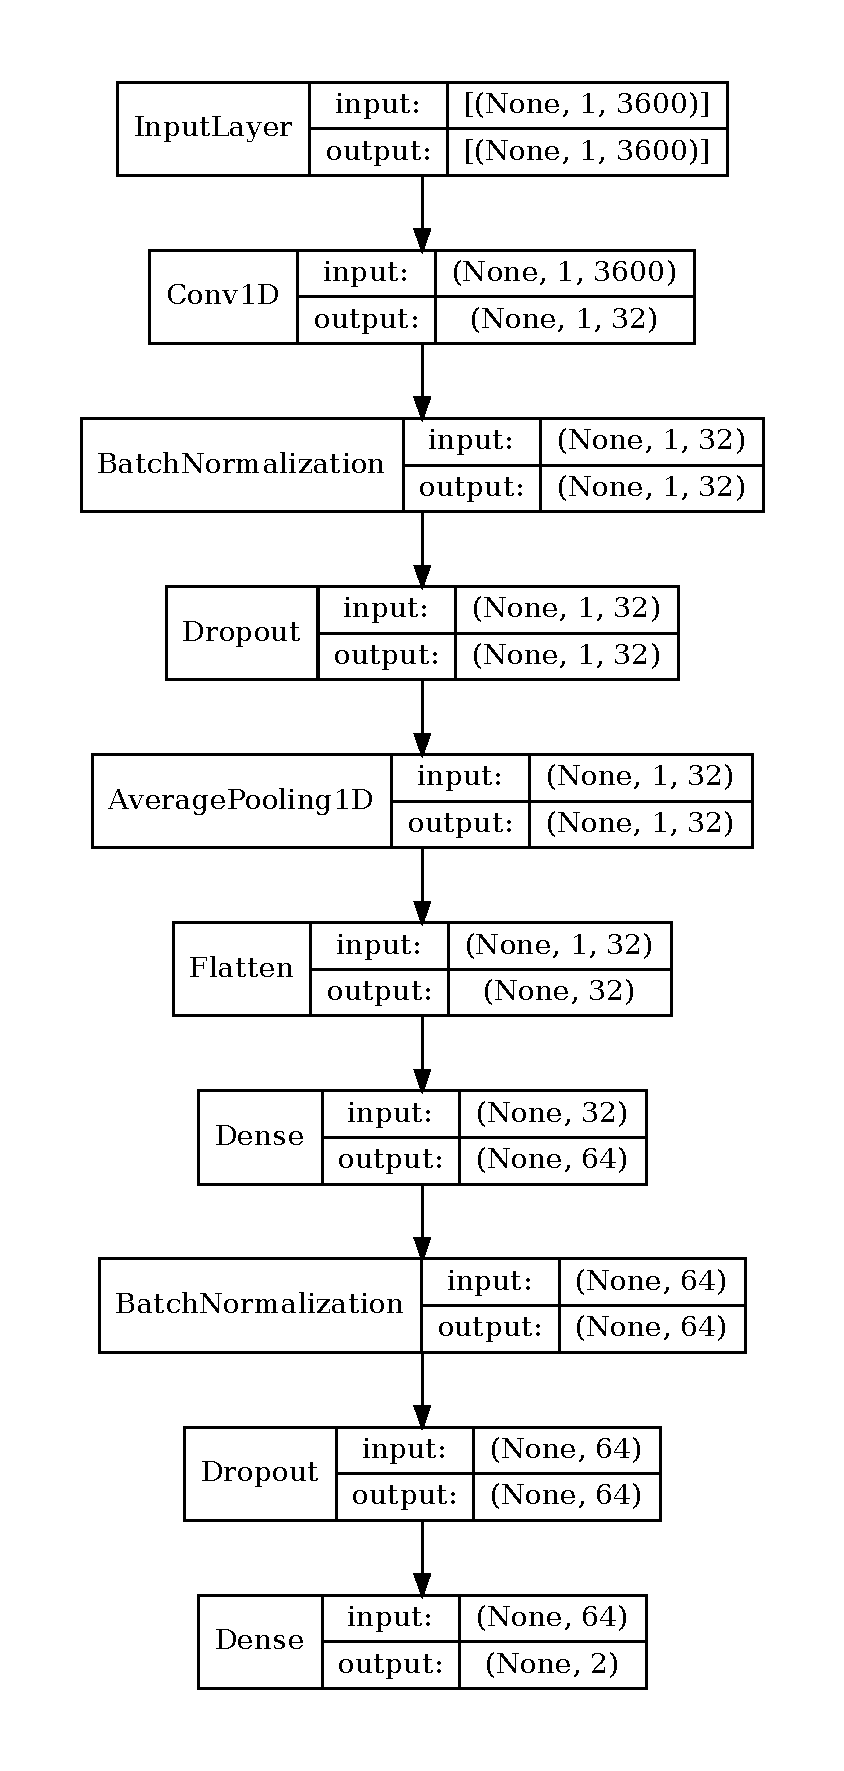
\includegraphics[width=\linewidth]{model_conv.pdf}
	\end{minipage}
	~
	\begin{minipage}{0.5\textwidth}
		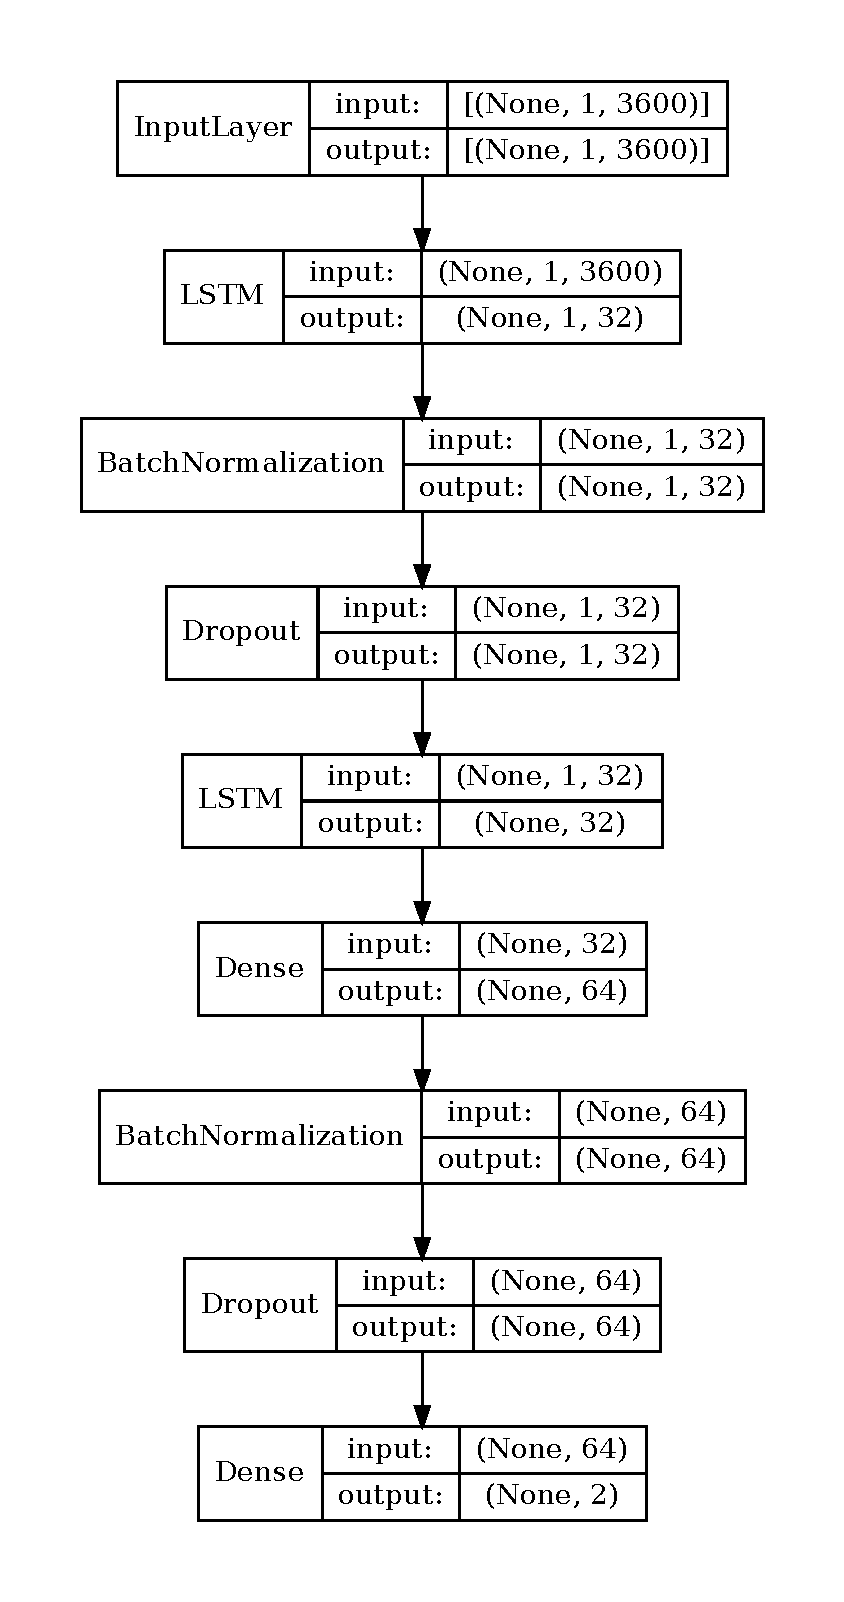
\includegraphics[width=\linewidth]{model_lstm.pdf}
	\end{minipage}
	\caption{Artificial neural networks from experiment. On the left-hand side is the 1D Convolutional ANN and on the right-hand side is the ANN with LSTM layers.}%
	\label{fig:arch_anns}
\end{figure}

\begin{lstlisting}[language=Python,label=list:code_ann1,caption=Implementation of 1D Convolutional ANN.,captionpos=b,frame=single,float]
model = Sequential([
  Conv1D(filters=32, kernel_size=8, strides=4,
    padding='same', activation=relu,
    input_shape=(inp_data.shape[1], inp_data.shape[2])),
  BatchNormalization(),
  Dropout(rate=0.3, seed=SEED),
  AveragePooling1D(
    pool_size=4, strides=1, padding='same'),
  Flatten(),
  Dense(64, activation=relu),
  BatchNormalization(),
  Dropout(rate=0.4, seed=SEED),
  Dense(2, activation=softmax),
])
model.compile(
  optimizer=Adam(learning_rate=0.001),
  loss=BinaryCrossentropy(),
  metrics=['acc', 'mae',
    tf.keras.metrics.Recall(),
    tf.keras.metrics.Precision()]
)
\end{lstlisting}

\begin{lstlisting}[language=Python,label=list:code_ann2,caption=Implementation of Long Short-Term Memory ANN.,captionpos=b,frame=single,float]
model = Sequential([
  LSTM(units=32, activation=relu,
    return_sequences=True),
  BatchNormalization(),
  Dropout(rate=0.3, seed=SEED),
  LSTM(units=32, activation=relu),
  Dense(64, activation=relu),
  BatchNormalization(),
  Dropout(rate=0.4, seed=SEED),
  Dense(2, activation=softmax),
])
model.compile(
  optimizer=Adam(learning_rate=0.001),
  loss=BinaryCrossentropy(),
  metrics=['acc', 'mae',
    tf.keras.metrics.Recall(),
    tf.keras.metrics.Precision()]
)
\end{lstlisting}

\begin{lstlisting}[language=Python,label=list:code_snn1,caption=Conversion of ANN model 1 to SNN model 3.,captionpos=b,frame=single,float]
converter = nengo_dl.Converter(
  model=model,
  swap_activations={
    tf.keras.activations.relu:
      nengo.SpikingRectifiedLinear()
  },
  scale_firing_rates=3000,
  synapse=0.1,
)
\end{lstlisting}

\begin{lstlisting}[language=Python,label=list:code_snn2,caption=SNN model with Legendre Memory Units.,captionpos=b,frame=single,float]
with nengo.Network(seed=SEED) as net:
  # input node for data
  inp = nengo.Node(np.ones(inp_data.shape[-1]))
  # LMU cell
  lmu1 = LMUCell(
    units=212,
    order=256,
    theta=inp_data.shape[-1],
    input_d=inp_data.shape[-1])
  lmu2 = LMUCell(
    units=212,
    order=256,
    theta=inp_data.shape[-1],
    input_d=212)
  # output node for probing result data
  out = nengo.Node(size_in=2)

  # input node is connected with LMU's `x` variable,
  # where input vectors flow into
  nengo.Connection(inp, lmu1.x, synapse=None)

  # LMU's hidden state is kept in a variable `h`
  # it is also an output connected to output node
  nengo.Connection(lmu1.h, lmu2.x,
    transform=nengo_dl.dists.Glorot(), synapse=None)

  nengo.Connection(lmu2.h, out,
    transform=nengo_dl.dists.Glorot(), synapse=None)

  # probe for collecting data
  p = nengo.Probe(target=out)
\end{lstlisting}

\newpage

%
% RESULTS
%

\section{Results}%
\label{sec:results}

Final results of all models with different averaging of \textit{brain signals} (the PV1, see Subsection~\ref{ssec:preproc_train} point 1) can be seen in Table~\ref{tab:results_signals}. Results of all models, that were fed with averaged random samples (the PV2, see Subsection~\ref{ssec:preproc_train} point 2) from artificially created dataset of size 10~000 samples can be seen in Table~\ref{tab:results_samples_10000} and results from models fed with the same way created dataset of size 20~000 are in Table~\ref{tab:results_samples_20000}.

In tables, there is accuracy, precision, recall and F1-score presented from previously mentioned collected metrics. Convolutional models were performing the best with accuracy of 63-64\% after PV1. After PV2, convolutional models were giving the best results again with accuracy of 64-66\%. This~accuracy was achieved with 10~000 artificial samples. But when the sample amount was doubled to 20~000, the accuracy increased to 65-68\%.

The transformed Convolutional ANN to Spiking Convolutional NN was always very close to original model with performance. When it outperformed the original model, it was by very small amount. LSTM network performed worse than 1D Convolutional network. And novel SNN with LMU neurons also did not outperform the convolutional networks. The LMU was actually the worst performing network, which was not expected, since it promises better performance than LSTM and since it is a spiking network, so it should handle one-dimensional input very well.

Generally PV1 did not have noticeable effect on the networks. With~PV2 the accuracy started increasing after a big amount of artificial samples. That can be seen in differences between Table~\ref{tab:results_samples_10000} and Table~\ref{tab:results_samples_20000}. But with growing averaging amount the accuracy started decreasing. That is very different result than in the original paper \cite{varekap300}, where accuracy was increasing. Accuracy of 70\% and more could not be achieved, unfortunately. Although, while training after PV2, training and validation accuracies were reaching up to 80\%.

% TABLE SIGNALS

\begin{table}[ht!]
	\centering
	\begin{tabular}{l c c c c c}
		\hline
		Model type & Averaging & Accuracy & Precision & Recall & F1-score \\
		\hline
		ANN 1D conv & None & 0.6383 & 0.6211 & 0.6770 & 0.6476 \\
		ANN LSTM    & None & 0.6305 & 0.6112 & 0.6856 & 0.6455 \\
		SNN 1D conv & None & \textbf{0.6391} & 0.6222 & 0.6767 & 0.6480 \\
		SNN LMU     & None & 0.5618 & 0.5743 & 0.4390 & 0.4956 \\
		\\
		ANN 1D conv & 3 & 0.6415 & 0.6271 & 0.6686 & 0.6468 \\
		ANN LSTM    & 3 & 0.6261 & 0.6057 & 0.6873 & 0.6433 \\
		SNN 1D conv & 3 & \textbf{0.6418} & 0.6271 & 0.6697 & 0.6474 \\
		SNN LMU     & 3 & 0.5715 & 0.5896 & 0.4215 & 0.4914 \\
		\\
		ANN 1D conv & 6 & \textbf{0.6424} & 0.6237 & 0.6872 & 0.6536 \\
		ANN LSTM    & 6 & 0.6286 & 0.6129 & 0.6655 & 0.6371 \\
		SNN 1D conv & 6 & 0.6422 & 0.6237 & 0.6865 & 0.6533 \\
		SNN LMU     & 6 & 0.5565 & 0.5630 & 0.4470 & 0.4972 \\
		\\
		ANN 1D conv & 9 & 0.6390 & 0.6203 & 0.6863 & 0.6511 \\
		ANN LSTM    & 9 & 0.6292 & 0.6100 & 0.6824 & 0.6436 \\
		SNN 1D conv & 9 & \textbf{0.6401} & 0.6199 & 0.6937 & 0.6541 \\
		SNN LMU     & 9 & 0.5711 & 0.5871 & 0.4344 & 0.4984 \\
		\hline
	\end{tabular}
	\caption{Results of P300 dataset classification with various ANNs and SNNs (models described in Table~\ref{tab:models} and with different averaging amounts of \textbf{features} in brain signals. For more about this averaging see Subsection~\ref{ssec:preproc_train} point 1.}
	\label{tab:results_signals}
\end{table}

% TABLE SAMPLES 10,000

\begin{table}[ht!]
	\centering
	\begin{tabular}{l c c c c c}
		\hline
		Model type & Averaging & Accuracy & Precision & Recall & F1-score \\
		\hline
		ANN 1D conv & 3 & \textbf{0.6680} & 0.6604 & 0.6839 & 0.6719 \\
		ANN LSTM    & 3 & 0.6472 & 0.6421 & 0.6628 & 0.6504 \\
		SNN 1D conv & 3 & 0.6678 & 0.6593 & 0.6806 & 0.6697 \\
		SNN LMU     & 3 & 0.5923 & 0.6127 & 0.4822 & 0.5384 \\
		\\
		ANN 1D conv & 6 & \textbf{0.6550} & 0.6613 & 0.6276 & 0.6437 \\
		ANN LSTM    & 6 & 0.6421 & 0.6337 & 0.6649 & 0.6487 \\
		SNN 1D conv & 6 & 0.6548 & 0.6596 & 0.6252 & 0.6417 \\
		SNN LMU     & 6 & 0.6008 & 0.6157 & 0.5203 & 0.5606 \\
		\\
		ANN 1D conv & 9 & \textbf{0.6540} & 0.6403 & 0.6948 & 0.6662 \\
		ANN LSTM    & 9 & 0.6405 & 0.6228 & 0.7018 & 0.6600 \\
		SNN 1D conv & 9 & 0.6535 & 0.6371 & 0.6972 & 0.6656 \\
		SNN LMU     & 9 & 0.6002 & 0.5951 & 0.6009 & 0.5978 \\
		\\
		ANN 1D conv & 12 & 0.6518 & 0.6466 & 0.6629 & 0.6540 \\
		ANN LSTM    & 12 & 0.6426 & 0.6269 & 0.6949 & 0.6591 \\
		SNN 1D conv & 12 & \textbf{0.6519} & 0.6451 & 0.6614 & 0.6524 \\
		SNN LMU     & 12 & 0.6090 & 0.6054 & 0.6060 & 0.6052 \\
		\\
		ANN 1D conv & 15 & \textbf{0.6497} & 0.6402 & 0.6753 & 0.6568 \\
		ANN LSTM    & 15 & 0.6380 & 0.6236 & 0.6907 & 0.6539 \\
		SNN 1D conv & 15 & 0.6493 & 0.6380 & 0.6744 & 0.6553 \\
		SNN LMU     & 15 & 0.5987 & 0.5923 & 0.6107 & 0.6009 \\
		\hline
	\end{tabular}
	\caption{Training data size 10~000 samples. Results of P300 dataset classification with various ANNs and SNNs (models described in Table~\ref{tab:models} and with different averaging amounts of \textbf{samples} among people. For more about this averaging see Subsection~\ref{ssec:preproc_train} point 2.}
	\label{tab:results_samples_10000}
\end{table}

% TABLE SAMPLES 20,000

\begin{table}[ht!]
	\centering
	\begin{tabular}{l c c c c c}
		\hline
		Model type & Averaging & Accuracy & Precision & Recall & F1-score \\
		\hline
		ANN 1D conv & 3 & \textbf{0.6877} & 0.6784 & 0.7078 & 0.6924 \\
		ANN LSTM    & 3 & 0.6624 & 0.6593 & 0.6643 & 0.6616 \\
		SNN 1D conv & 3 & 0.6876 & 0.6767 & 0.7069 & 0.6911 \\
		SNN LMU     & 3 & 0.5900 & 0.6174 & 0.4536 & 0.5222 \\
		\\
		ANN 1D conv & 6 & \textbf{0.6760} & 0.6659 & 0.6996 & 0.6821 \\
		ANN LSTM    & 6 & 0.6577 & 0.6566 & 0.6557 & 0.6554 \\
		SNN 1D conv & 6 & 0.6758 & 0.6639 & 0.6990 & 0.6807 \\
		SNN LMU     & 6 & 0.6008 & 0.6157 & 0.5203 & 0.5606 \\
		\\
		ANN 1D conv & 9 & \textbf{0.6613} & 0.6482 & 0.6983 & 0.6718 \\
		ANN LSTM    & 9 & 0.6523 & 0.6466 & 0.6648 & 0.6551 \\
		SNN 1D conv & 9 & 0.6609 & 0.6458 & 0.6983 & 0.6705 \\
		SNN LMU     & 9 & 0.6002 & 0.5951 & 0.6009 & 0.5978 \\
		\\
		ANN 1D conv & 12 & \textbf{0.6589} & 0.6505 & 0.6794 & 0.6643 \\
		ANN LSTM    & 12 & 0.6478 & 0.6346 & 0.6885 & 0.6602 \\
		SNN 1D conv & 12 & 0.6586 & 0.6483 & 0.6789 & 0.6629 \\
		SNN LMU     & 12 & 0.6090 & 0.6054 & 0.6060 & 0.6052 \\
		\\
		ANN 1D conv & 15 & \textbf{0.6525} & 0.6455 & 0.6683 & 0.6565 \\
		ANN LSTM    & 15 & 0.6406 & 0.6254 & 0.6922 & 0.6567 \\
		SNN 1D conv & 15 & 0.6524 & 0.6434 & 0.6682 & 0.6554 \\
		SNN LMU     & 15 & 0.5987 & 0.5923 & 0.6107 & 0.6009 \\
		\hline
	\end{tabular}
	\caption{Training data size 20~000 samples. Results of P300 dataset classification with various ANNs and SNNs (models described in Table~\ref{tab:models} and with different averaging amounts of \textbf{samples} among people. For more about this averaging see Subsection~\ref{ssec:preproc_train} point 2.}
	\label{tab:results_samples_20000}
\end{table}
